\documentclass[11pt]{article}
\title{\textbf{Microbiologia}}
\author{Simona Debilio}
\date{}

\usepackage{graphicx}
\usepackage[utf8x]{inputenc}
\usepackage[italian]{babel}
\setlength{\parindent}{0pt}


\begin{document}

\maketitle

\tableofcontents

\clearpage

\section{Struttura e funzione di una cellula procariote}

Con il termine \emph{``microrganismo''} si indicano organismi dalle dimensioni molto piccole che possono essere sia procarioti che eucarioti (lieviti, muffe, ecc...).
Questi due tipi cellulari condividono alcune caratteristiche:
\begin{itemize}
\item Tutte le cellule presentano una membrana plasmatica;
\item Il citoplasma ha una composizione simile;
\item Entrambe possiedono ribosomi (la composizione e il peso di quest'ultimi però variano tra le due).
\end{itemize}
\vspace{1em}
Caratteristiche distintive dei \emph{procarioti}:
\begin{itemize}
\item Sono organismi unicellulari;
\item La cellula procariote non ha organelli cellulari oltre ai ribosomi;
\item Non possiedono mitocondri, l'energia viene prodotta a livello della membrana cellulare;
\item Hanno maggiore semplicità strutturale e minori dimensioni della cellula;
\item La divisione cellulare avviene tramite la scissione binaria.
\end{itemize} 
\vspace{1em}
I procarioti si dividono in due grandi gruppi:
\begin{enumerate}
\item \textbf{Batteri};
\item \textbf{Archea}.
\end{enumerate}
\vspace{1em}
Nei batteri si trova un unico cromosoma circolare.
Avendo poco spazio all'interno della cellula, il 98\% del materiale genetico dei batteri è codificante (non sono presenti gli istoni).
\\Nei procarioti è possibile che ci sia del materiale genetico accessorio (come ad esempio i plasmidi) autoreplicante, cioè indipendente dal cromosoma per la sua replicazione, che apporta al batterio capacità accessorie (virulenza, resistenza alla salinità, resistenza gli antibiotici...).\\

La \textbf{parete cellulare} nei batteri è formata da \textbf{peptidoglicano} (mai presente negli eucarioti).
I batteri possiedono dei \textbf{flagelli} che gli permettono di muoversi: un batterio dotato di flagelli è molto più aggressivo perché è in grado di spostarsi in altre zone più adatte alla vita.
I batteri presentano anche dei \textbf{pili} (utilizzati nella coniugazione).\\

Il peptidoglicano è tipico della parete dei batteri, mentre gli Archea possiedono uno \textbf{pseudopeptidoglicano}.
A differenza dei batteri, gli Archea possono crescere a temperature superiori ai 100 gradi.\\

Le dimensioni standard della cellula batterica vanno dagli 0,2 ai 2 micron.
La cellula modello è quella di E. Coli.\\

Esistono delle dimensioni ottimali per il batterio: dimensioni piccole infatti consentono alla cellula di poter effetturare scambi più efficienti con l'esterno. Inoltre, le dimensioni influenzano il tasso di trasporto di nutrienti e prodotti di scarto del metabolismo attraverso la cellula.\\

Aumentando le dimensioni aumenta anche il rapporto tra la superficie ed il volule cellulare rendendo gli scambi con l'esterno meno efficienti.\\

I batteri possono essere suddivisi, in base della loro forma, in:
\begin{itemize}
\item \textbf{Cocchi}, dalla forma sferica;
\item \textbf{Bacilli}, dalla forma a bastoncino;
\item \textbf{Coccobacilli}, dalla forma intermedia tra cocchi e bacilli.
\end{itemize}
\clearpage
A seconda del tipo di divisione effettuata dai cocchi poi, si possono riconoscere:
\begin{itemize}
\item \textbf{Diplococchi} o \textbf{streptococchi}, se il cocco si divide secondo \emph{un} piano verticale;
\item \textbf{Tetradi}, se il cocco si divide secondo \emph{due} piani verticali e uno orizzontale;
\item \textbf{Sarcine}, se il cocco si divide secondo \emph{due piani verticali e uno orizzontale};
\item \textbf{Stafilococchi}, se i cocchi si dividono in maniera disordinata.
\end{itemize}

\vspace{1em}
Oppure possono assumere forme ricurve, e allora vengono suddivisi in:
\begin{itemize}
\item \textbf{Vibrione}, dalla forma a bastoncino leggermente ricurvo;
\item \textbf{Spirilli}, dalla forma più ricurva rispetto ai vibrioni;
\item \textbf{Spirocheti}, dalla forma quasi ad elica.
\end{itemize}
Ciò che cambia è la flessibilità del batterio: le spirochete sono più flessibili dei vibrioni.\\

Esistono poi altri due tipi di batteri:
\begin{itemize}
\item I \textbf{batteri prostecati}, i quali possiedono un peduncolo di adesione al substrato;
\item I \textbf{batteri filamentosi}, formati da ife e micelio.
\end{itemize}

\vspace{1em}
Dalla divisione cellulare del \emph{Caulobacter}, un batterio prostecato, si ottengono due cellule attaccate l'una all'altra di cui una presenta un peduncolo e l'altra presenta un flagello. \\Successivamente la cellula con il flagello si stacca e forma una cellula a parte.\\

I batteri presentano proteine simili a quelle del citoscheletro delle cellule eucarioti regolano la forma e la dimensione delle cellule batteriche durante l'accrescimento.
\\Ad esempio:
\begin{itemize}
\item \textbf{FtsZ}, nei cocchi, si concentra in posizione mediana e coordina la formaizone della nuova parete cellulare che separerà le due cellule;
\item \textbf{MreB}, nei bastoncelli, forma una struttura elicoidale a livello della membrana plasmatica;
\item \textbf{CreS} (detta "crescentina") è responsabile della curvatura della cellula.
\end{itemize}

\section{Il rivestimento della cellula batterica}

La cellula procariote presenta complesse strutture di rivestimento che consentono al batterio di adattarsi a condizioni ambientali anche estreme.

Tutte le cellule procariote presentano una membrana plasmatica che separa l'interno della cellula dall'esterno. 

In generale i batteri presentano anche una parete che ha composizione e posizione diversa a seconda del gruppo microbico.

Possono poi essere presenti altre strutture di rivestimento (strato S, capsula, glicocalice...) e appendici di superficie (pili e flagelli).

I batteri che presentano la capsula sono particolarmente virulenti perché protetti molto bene e dunque molto resistenti.

\subsection{Differenze nella composizione dell'involucro esterno tra batteri Gram+ e Gram-}
I batteri \textbf{Gram+} presentano (partendo dall'interno):
\begin{itemize}
\item Una membrana plasmatica a doppo strato fosfolipidico;
\item Un sottile strato detto periplasma in cui vengono riversati enzimi e in cui avvengono reazioni metaboliche;
\item Uno strato spesso di peptidoglicano.
\end{itemize}

I \textbf{Gram-} presentano (partendo dall'interno):
\begin{itemize}
\item una membrana plasmatica;
\item un periplasma spesso in cui è immerso un sottile strato di peptidoglicano;
\item una membrana esterna (diversa chimicamente dalla membrana plasmatica).
\end{itemize}

\begin{figure}[htp]
\centering
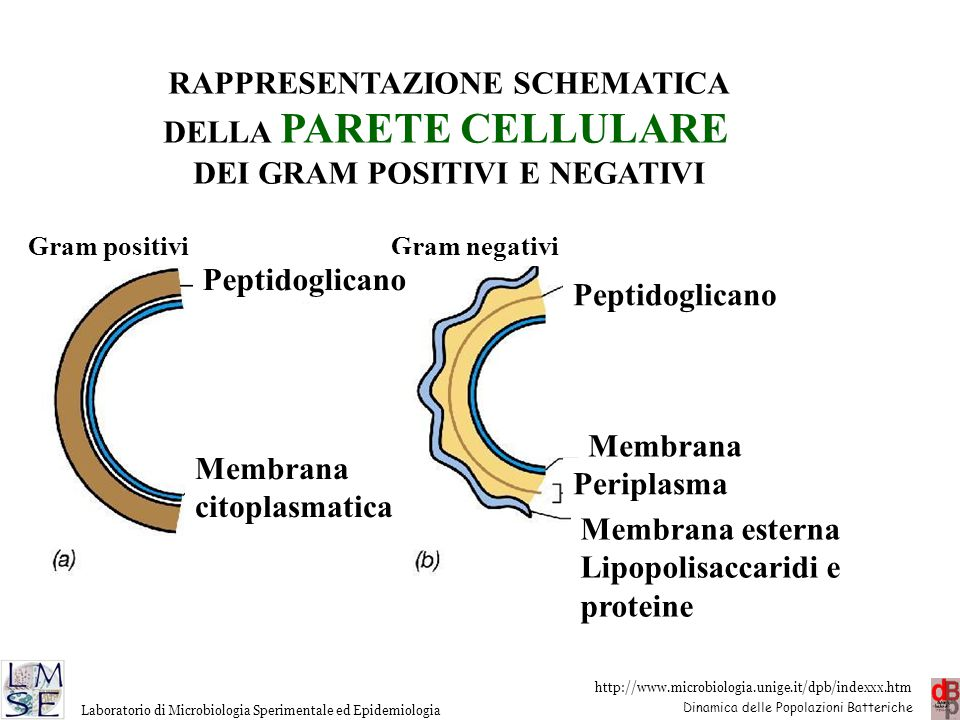
\includegraphics[scale=0.40]{img/parete_cellulare.jpg}
\caption{Differenze nella membrana tra batteri Gram+ e Gram-}
\label{parete_cellulare}
\end{figure}

\subsubsection{Composizione della membrana plasmatica}
Nei batteri la membrana plasmatica è formata da una membrana fosfolipidica classica: un doppio strato fosfolipidico organizzato con le teste polari rivolte verso l'esterno e le code idrofobiche rivolte verso l'interno.\\

Esistono tuttavia delle differenze nella composizione tra la membrana dei Bacteria e quella degli Archea.\\

Nei \textbf{Bacteria}:
\begin{itemize}
\item La \emph{testa} del fosfolipide è formata da una molecola di \textbf{D-glicerolo-3-fosfato}. Al fosfato esterificato al C3 possono essere legati dei gruppi funzionali;
\item La \emph{coda} è costituita da \textbf{due molecole di acidi grassi esterificati} al C1 e C2 (in maggioranza sono \textbf{saturi}, con aggiustamenti dettati da variazioni ambientali);
\item Il gruppo fosfato è esterificato sul \textbf{C3}.
\end{itemize}

\vspace{1em}
Tipicamente, nelle membrane dei Bacteria sono assenti gli steroli (con l'eccezione dei metilotrofi), come il colesterolo, i quali sono sostituiti dagli \textbf{opanoidi}.
Gli opanoidi contribuiscono a stabilizzare la struttura e a renderla meno flessibile (svolgono la stessa funzione del colesterolo nelle cellule eucariote).\\

Negli \textbf{Archea}:
\begin{itemize}
\item La testa del fosfolipide è formata da una molecola di \textbf{L-glicerolo-3-fosfato}. I legami con le catene idrofobiche si formano al C2 e al C3;
\item Negli Archea il legame tra il glicerolo e le catene alifatiche, ovvero le catene di acidi grassi, sono \textbf{eteri} (e NON esteri)
\item Il gruppo fosfato è esterificato sul \textbf{C1};
\item Negli Archea le catene di acidi grassi sono costituite da catene di \textbf{isoprene} contenenti doppi legami.
\end{itemize}


\begin{figure}[htp]
\centering
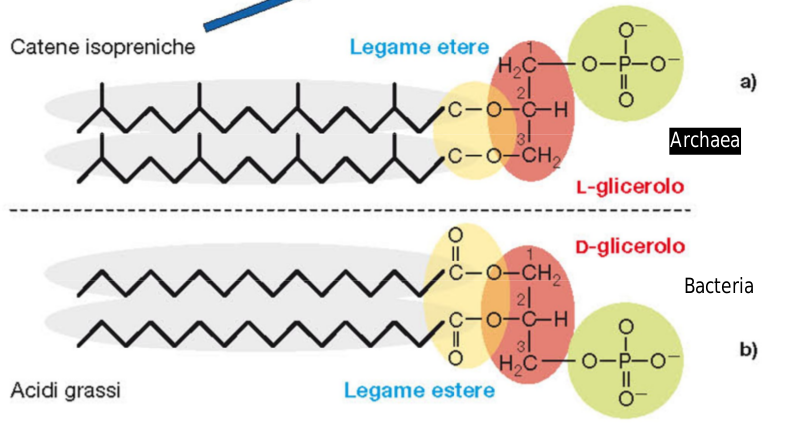
\includegraphics[scale=0.3]{img/Fosfolipidi.png}
\caption{Differenze nei fosfolipidi di Bacteria e Archea}
\label{}
\end{figure}

\vspace{1em}
I lipidi degli Archea possono essere \textbf{dieteri} (cioè con 2 catene alifatiche a 20C legate covalentemente al glicerolo) o \textbf{tetraeteri} (cioè 2 catene alifatiche a 40C legate a due molecole di glicerolo) del glicerolo. 

Negli Archea a volte non è presente un doppio strato fosfolipidico, ma un monostrato fosfolipidico il quale garantisce una maggiore stabilità alle membrane (si trova frequentemente negli Archea ipertermofili).

Questo monostrato si forma perché a volte la coda di \textbf{fitanile} di una molecola si collega alla coda di fitanile di un'altra molecola formando così un'unica molecola di \textbf{bifitanile} che fa sì che non ci sia più un doppio strato ma uno strato unico.

\begin{figure}[htp]
\centering
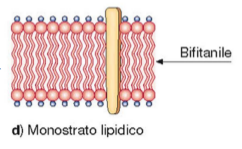
\includegraphics[scale=0.8]{img/Bifitanile.png}
\caption{Monostrato fosfolipidico}
\label{}
\end{figure}

Nelle membrane plasmatiche dei batteri, come in quelle eucaristiche, sono presenti anche delle proteine.
Queste possono svolgere ruoli di diverso tipo: possono formare canali, possono essere sensori di membrana, possono essere lipoproteine (nei Gram+ sono esposte verso l'esterno e nei Gram- sono esposte verso il periplasma), ecc...\\

Nella membrana di \emph{E. Coli} sono presenti oltre 200 tipi di proteine

\subsubsection{Funzioni della membrana plasmatica}
\begin{itemize}
\item \textbf{Regolare la permeabilità}, rappresenta una barriera attraversabile solo da molecole piccole e non cariche e da molecole idrofobiche tramite diffusione;
\item \textbf{è il sito in cui sono collocate alcune proteine} che possono regolare il trasporto (formando canali), oppure possono modificare e trasferire un segnale alla cellula...;
\item \textbf{Produzione di energia}, respirazione e fotosintesi avvengono a livello di membrana. In entrambi i processi viene generato un gradiente ionico transmembrana (detta forza proton-motrice) che viene utilizzato dalla cellula per sintetizzare ATP;
\item \textbf{Biosintesi di componenti cellulari} come fosfolipidi, parti del peptidoglicano e del lipopolisaccaride.
\end{itemize}

\subsection{La parete batterica}

La parete batterica si differenzia per posizione e spessore tra Gram+ e Gram-: nei Gram+ è spessa, mentre nei Gram- è sottile e immersa nel periplasma.

Esternamente alla membrana citoplasmatica si trova una molecola polimerica chiamata \textbf{peptidoglicano} o \textbf{mureina}, la quale avvolge la cellula conferendole rigidità e forma.\\
Il peptidoglicano è formato da catene glicaniche costituite da due aminozuccheri alternati:
\begin{itemize}
\item il \textbf{NAG} (N-acetil glucosammina);
\item il \textbf{NAM} (Acido N-acetil muramico). Al NAM è legato un \emph{tetrapeptide} tramite il quale le catene glicaniche si connettono.
\end{itemize}

Tra questi due zuccheri vi è un legame $\beta$ 1-4 glucosidico che li lega in maniera successiva formando così delle lunghe catene.

\vspace{1em}
Legata al NAM, come già detto, c’è una catena di 4 amminoacidi. Per conferire ordine e resistenza alla struttura, il 3° amminoacido del NAM di una catena NAM-NAG si lega al 4° amminoacido del NAM di una catena parallela (questa viene detta struttura base).

\begin{figure}[htp]
\centering
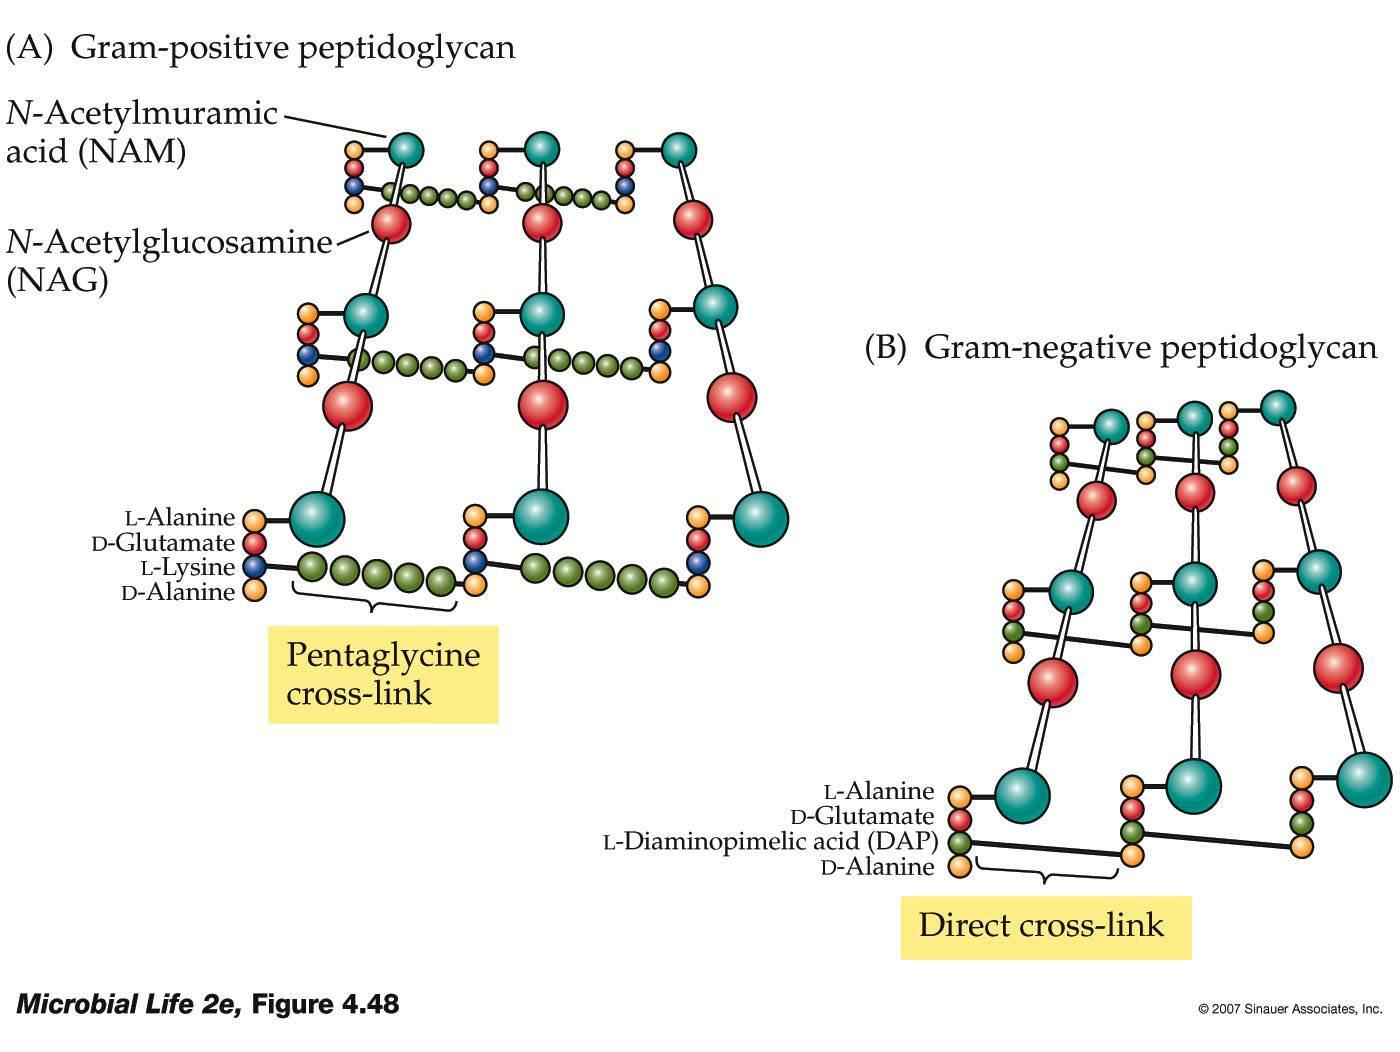
\includegraphics[scale=0.2]{img/NAM_NAG.jpg}
\caption{Legami nella parete cellulare}
\label{Legami parete cellulare}
\end{figure}


\clearpage
I Gram+ hanno una struttura più forte del peptidoglicano e resistono a temperature elevate più dei Gram-.\\
Questo avviene perché i Gram+ e i Gram- presentano delle differenze nel peptidoglicano: mentre nei Gram- il 3° e il 4° amminoacido sono legati direttamente tra loro, nei Gram+ il legame crociato non è diretto direttamente tra il 3° e il 4° amminoacido ma tra i due amminoacidi è inserita una \textbf{catena di pentaglicina}.\\
Un’altra differenza consiste nella sequenza dei 4 amminoacidi che per i G+ sono: 
\begin{enumerate}
\item L-Alanina;
\item D-Glutammato;
\item L-Lisina;
\item D-Alanina.
\end{enumerate}

Mentre nei G- i 4 amminoacidi sono:
\begin{enumerate}
\item L-Alanina;
\item D-Glutammato;
\item Acido L-Diaminopimelico (DAP);
\item D-Alanina.
\end{enumerate}

Questo significa che nei Gram+ il legame tra le catene avviene tra la lisina di una catena e l’alanina dell’altra, mentre nei Gram - il legame avviene tra l’acido L-Diaminopimelico e l’alanina.

\vspace{2em}
Il \textbf{lisozima} è un enzima presente nelle secrezioni biologiche come la saliva e le lacrime.
Questo enzima espleta un'azione antimicrobica grazie alla capacità di idrolizzare i peptidoglicani che formano la parete batterica. Il lisozima infatti è in grado di colpire i legami $\beta$ 1-4 tra gli zuccheri NAM e NAG.\\
In seguito alla lesione del peptidoglicano la cellula batterica inizia a richiamare acqua fino a scoppiare.


\subsubsection{La biosintesi del peptidoglicano}

la biosintesi del peptidoglicano avviene in tre differenti comparti della cellula:
\begin{enumerate}
\item nel \textbf{citoplasma}, dove vengono sintetizzati i \emph{precursori};
\item nella \textbf{membrana citoplasmatica}, dove avviene la sintesi dell’unità monomerica del glicano legato a un trasportatore lipidico e il suo ribaltamento sulla faccia esterna della membrana citoplasmatica;
\item nello \textbf{spazio esterno alla membrana} dove avvengono reazioni di polimerizzazione e transpeptidazione (si formano i legami crociati).
\end {enumerate}

La sintesi del NAG proviene da una trasformazione del \emph{Fruttosio-6-fosfato} con \emph{UTP} da cui si genera una molecola chiamata \textbf{UDP-NAG}.\\
A questo punto una molecola di \emph{PEP} viene trasferita al gruppo -OH dell’UDP-NAG da parte di \textbf{Mur A} formando un intermedio che viene poi trasformato da \textbf{Mur B} a \textbf{UDP-NAM}. \\
A questo punto intervengono altri enzimi chiamati \textbf{Mur C}, \textbf{Mur D}, \textbf{Mur E} e \textbf{Mur F}, i quali sono \emph{ligasi} responsabili dell’attacco della catena di amminoacidi al NAM (in questo momento gli amminoacidi sono 5, c’è un’Alanina supplementare).

\begin{figure}[htp]
\centering
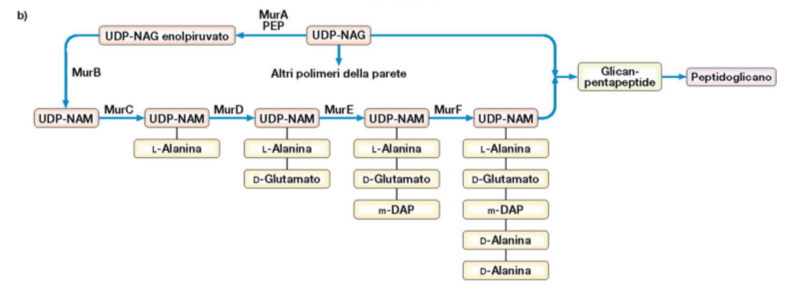
\includegraphics[scale=0.4]{img/Assemblaggio NAM.png}
\caption{Assemblaggio NAM}
\label{}
\end{figure}

A livello della faccia interna della membrana, si trova un trasportatore chiamato \textbf{bactoprenolo} (alcol a 55 C, idrofobo) che \emph{lega il NAM-pentammide} formando il \textbf{lipide I}. Successivamente al lipide I si lega un NAG e si forma il \textbf{lipide II}. A questo punto il bactoprenolo si ribalta sul lato esterno della membrana e diventa un substrato di \emph{transglicosilasi} che catalizza il legame tra il monomero nascente e il filamento nascente.\\
Successivamente si forma il legame peptidico tra la catena pentapeptidica del nuovo monomero e il tetrapeptide di una catena di glicano adiacente ad opera di \textbf{transpeptidasi}. \\
Infine il bactoprenolo viene defosforilato e ribaltato nuovamente sulla faccia interna della membrana.

\begin{figure}[htp]
\centering
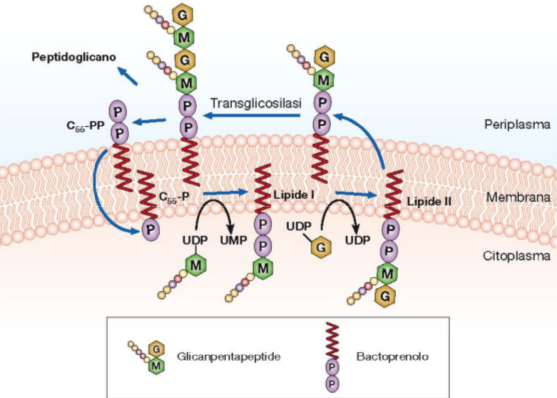
\includegraphics[scale=0.5]{img/Biosintesi peptidoglicano.png}
\caption{Biosintesi peptidoglicano}
\label{}
\end{figure}


\vspace{1em}
Tutta questa è una struttura molto complessa che ha dei punti deboli sui quali possono agire molti antibiotici. Ad esempio:
\begin{itemize}
\item la transpeptidazione può essere inibita da penicciline e cefalosporine;
\item la Bacitracina inibisce la defosforilazione del bactoprenolo;
\item cicloserina, inibisce la trasformazione di L-alanina in D-alanina...
\end{itemize}

Il peptidoglicano è presente unicamente nelle cellule batteriche. Per questo motivo gli antibiotici che vanno ad intaccare il peptidoglicano hanno una bassa tossicità: essi non possono intaccare le nostre cellule eucariotiche poiché esse non possiedono il peptidoglicano.

\subsubsection{La parete batterica dei Gram+}

Il rivestimento della cellula batterica dei Gram+, ovvero la parete batterica, costituisce il 40 \% del peso secco della cellula e ha uno spessore di 50 nm.\\
Contiene \textbf{acidi teicoici} e \textbf{lipoteicoici} i quali sono polimeri anionici.\\
Gli \emph{acidi teicoici} costituiscono il 60\% della parete cellulare e si legano covalentemente allo scheletro polisacccaridico del peptodoglicano. Gli \emph{acidi lipoteicoici} invece, prendono contatto con la membrana citoplasmatica.
Queste molecole contribuiscono a fornire caratteri chimico fisici all’involucro, conferiscono carica superficiale negativa alla parete, e controllano il movimento degli ioni e dei cationi metallici.

\vspace{1em}
L'involucro esterno è costituito da una membrana a doppio strato e da uno spesso strato di peptidoglicano. Al peptidoglicano sono associati degli acidi che si differenziano per posizione, poichè quelli \emph{teicoici} sono immersi nel peptidoglicano mentre quelli \emph{lipoteicoici} fuoriescono dalla membrana. \\
Questi acidi hanno il compito di conferire alla cellula una carica negativa che consente al batterio di aderire alle argille grazie a interazioni elettrostatiche.\\
Mancano della membrana esterna.


\subsubsection{La parete batterica dei Gram-}
Il rivestimento della cellula battericadei Gram-, ovvero la parete batterica, consiste di un ottile strato di peptidoglicano circondato da una membrana esterna a doppio strato fosfolipidico. Questa membrana esterna tuttavia, ha una composizione diversa rispetto alle altre membrane biologiche.\\
Lo spazio compreso tra la membrana citoplasmatica e la membrana esterna viene chiamato \textbf{periplasma}

\vspace{1em}
Il preplasma è un comparto acquoso che può rappresentare il 20-40\% del volume cellulare totale.

\clearpage
Al suo interno sono presenti proteine periplasmatiche coinvolte in: 
\begin{itemize}
\item acquisizione di nutrienti:
\item generazione di energia;
\item sintesi del peptidoglicano;
\item biogenesi della membrana esterna;
\item degradazione e inattivazione degli antibiotici.
\end{itemize}


\vspace{2em}
La \textbf{membrane esterna} è particolare e viene detta asimmetrica poichè perchè presenta due strati con differente composizione: lo strato rivolto verso l'interno è formato da \textbf{fosfolipidi}, mentre lo strato esterno è formato da \textbf{lipopolisaccaridi (LPS) }in cui sono immerse le proteine di transmembrana.\\

I \emph{lipopolisaccaridi} sono molecole anfipatiche contenenti lipidi e residui saccaridici.\\
Questa molecola è costituita da:
\begin{itemize}
\item un \textbf{lipide A}, ovvero un \emph{dimero di NAG esterificato con due gruppi fosfato e 4-7 molecole di acido grasso};
\item un \textbf{Core}, ovvero una regione polisaccaridica suddivisa in 
\begin{itemize}
\item un \textbf{core interno}, una regione conservata contenente 1-3 molecole di \textbf{2-cheto-3-deossiottonato (Kdo)} e uno \emph{zucchero a 7C};
\item un \textbf{core esterno} dalla composizione variabile contenente zuccheri a 6-7C; 
\end{itemize}
\item un \textbf{Antigene O}, ovvero un \emph{polisaccaride} costituito da unità tetra o pentasaccaridiche che si estendono fuori dalla cellula.
\end{itemize}

Grazie ai gruppi fosfato e agli zuccheri carichi la superficie esterna è carica negativamente.

\vspace{1em}
L'antigene stimola la risposta immunitaria poiché quando entrano i microrganismi il sistema immunitario dell'organismo ospite reagisce con la produzione di anticorpi specifici.
Nei batteri patogeni l’LPS rappresenta dunque un fattore di virulenza in grado di evadere le barriere aspecifiche dell’ospite (fagocitosi e attivazione del complemento).\\
La \emph{catena laterale O} induce nell’ospite la produzione di anticorpi specifici, mentre il \emph{lipide A} attiva l’immunità innata con conseguente produzione di citochinine e risposta infiammatoria.

\vspace{1em}
Nella membrana esterna inoltre sono presenti:
\begin{itemize}
\item \textbf{porine}, complessi costituiti da tre monomeri di proteine transmembrana con struttura a botte ($\beta$ barrel) la cui cavità centrale costituisce il canale, dotato di diametro variabile, attraverso il quale fluiscono molecole più o meno grandi;
\item \textbf{lipoproteine} che stabilizzano la membrana e sono coinvolte nel trasporto di nutrienti, nella resistenza agli antibiotici e nella trasduzione del segnale.
\end{itemize}

\subsubsection{La colorazione di Gram}
La colorazione di Gram si basa su 4 passaggi in cui si ha l’utilizzo di:
\begin{enumerate}
\item un colorante (cristal-violetto);
\item un fissante (LUGOL);
\item un preparato in proporzioni variabili di alcol e acetone;
\item un decolorante; 
\item un colorante di contrasto (safranina).
\end{enumerate}

\textbf{Procedimento}\\
Dopo aver formato una coltura di batteri:
\begin{enumerate}
\item toccare a colonia batterica con un bastoncino e stemperare la colonia rimasta sul bastoncino su un vetrino con una goccia d’acqua;
\item effettuare la fissazione al calore: passare il vetrino con i batteri e l’acqua su una fiamma per farne evaporare l’acqua. I batteri in questo modo muoiono e rimangono adesi al vetrino;
\item versare delle gocce di colorante cristal-violetto sul preparato. Questo colorante entra sia nei batteri G+ che in quelli G- conferendogli il colore viola;
\item fissare il colore tramite qualche goccia il LUGOL, dopodiché lavare le cellule per toglierne l’eccesso;
\item fissare il colore con il preparato di alcol-acetone. Questa soluzione entra solo nelle batteri Gram - decolorandoli, mentre non riesce ad entrare nei Gram+ a causa del peptidoglicano che, insieme al colorante, forma uno strato impermeabile;
\item aggiungere il colorante di contrasto, la safranina, che colora solo i batteri Gram -.
\end{enumerate}

\begin{figure}[htp]
\centering
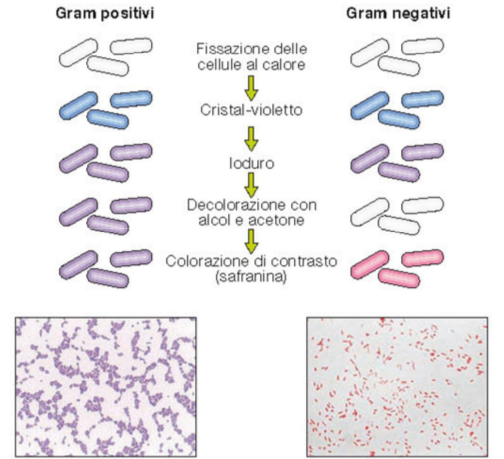
\includegraphics[scale=0.5]{img/Colorazione di Gram.png}
\caption{Colorazione di Gram}
\label{}
\end{figure}

Esistono poi dei batteri che vengono detti \textbf{Gram variabili}.\\
Alcuni batteri Gram+ (Arthrobacter, Actinomyces, Corynebacterium, Mycobacterium e Propionibacterium) infatti, rispondono in modo diverso alla colorazione di Gram in base alla loro fase di crescita: da giovani si colorano in maniera corretta, cioè esattamente come si colorerebbero i Gram+, mentre in una fase di crescita avanzata questi batteri assumono la colorazione dai Gram-. Questo avviene perché colture in fase di crescita più avanzata sono più fragili a livello del setto di divisione e rilasciano più facilmente il colorante.


\subsubsection{La parete batterica degli Archea}
Gli Archea non possiedono un vero peptidoglicano ma uno \textbf{pseudopeptidoglicano} (o pseudomureina) in cui il NAM è sostituito dal \textbf{NAT (Nacetil-talosaminuronico)} collegato a catene laterali di \emph{L-aminoacidi} (nel peptidoglicano sono presenti anche D-aminoacidi).\\
Gli amminozuccheri sono uniti da un legame $\beta$-1,3 anziché $\beta$-1,4.\\
Gli Archaea presentano una composizione di parete variabile a seconda del tipo di ambiente in cui vivono.

\subsection{Rivestimenti esterni delle cellule batteriche}
\subsubsection{Lo strato S o S layer}

Al di sopra dell’involucro esterno delle cellule batteriche, a volte, si può trovare lo strato S (o S layer).
Gli strati S sono costituiti da proteine insolubili in acqua che si assemblano a formare un reticolo cristallino di 5-25 nm. Le proteine che formano questo strato sono debolmente acide e legate a catene di glicani che sporgono all’esterno della cellula.\\
Di preciso non si sa che funzioni svolga questo strato ma certamente costituisce una barriere protettiva, promuove l’adesione cellulare, mantiene la rigidità cellulare, e nei batteri patogeni protegge dai meccanismi di difesa dell’ospite.\\
La capacità di un batterio di aderire al substrato può avere una notevole importanza clinica perché questi batteri possono aderire ai “medical devices” (come i cateteri) e causare infezioni nei pazienti.

\vspace{1em}
Lo stato S, a seconda della cellula batterica in cui si forma, può essere associato a diverse strutture della parete batterica:
\begin{itemize}
\item nei \emph{Gram+} e negli Archea è appoggiato al peptidoglicano;
\item nei \emph{Gram-} è appoggiato alla membrana esterna;
\item nei \emph{batteri privi} della parete cellulare lo strato S si appoggia direttamente alla membrana plasmatica (es. di batteri senza parete: i citoplasmi. Questi sono agenti patogeni che vivono nel floema delle piante, sono batteri vascolari e appartengono ad un gruppo tassonomico detto Mollicutes).
\end{itemize}
 
\subsubsection{Il glicocalice e la capsula}

Molti batteri rilasciano polisaccaridi che aderiscono alla superficie cellulare formando uno strato mucoso detto \textbf{glicocalice}. 
Se il glicocalice è ben strutturato e adeso alla parete cellulare viene definito \emph{capsula}, altrimenti, viene definito come \emph{slime layer}.\\ 
Batteri dotati di capsula hanno fenotipo mucoso, quelli privi di capsula hanno fenotipo rugoso.\\
Anche la capsula e il glicocalice svolgono un compito di protezione dell’organismo impedendogli d’entrare in contatto con le molecole antibiotiche, e proteggendoli dalla fagocitosi da parte di protozoi e di cellule del sistema immunitario.\\
Inoltre costituiscono un fattore di virulenza, e promuovono l’adesione ai substrati.

\vspace{1em}
La presenza della capsula può essere identificata tramite una colorazione negativa

\section{Il movimento dei batteri}

I batteri si muovono nuotando, sciamando, strisciando, contraendosi o galleggiando grazie a strutture esterne o interne (flagelli, pili, proteine del citoscheletro, vescicole gassose o magnetosomi).\\
Queste strutture sono alla base di vari fenomeni di \textbf{tassia} che regolamentano il movimento dell'organismo verso siti favorevoli:
\begin{itemize}
\item \textbf{chemiotassi}, ovvero un movimento in risposta a stimoli chimici. Può essere: \emph{positiva}, se è presente una molecola gradita al batterio, o \emph{negativa} se il batterio si allontana in risposta ad una molecola dannosa;
\item \textbf{fototassi}, ovvero un movimento verso certe lunghezze d’onda della luce. È un movimento tipico dei batteri fotosintetici;
\item \textbf{aerotassi}, un movimento in risposta alla concentrazione dell’ossigeno;
\item \textbf{magnetotassi}, un movimento lungo linee di forza magnetiche;
\item \textbf{pHtassi}, un movimento in risposta al pH;
\item \textbf{termotassi}, un movimento verso una temperatura ottimale;
\item \textbf{osmotassi}, un movimento in risposta a concentrazioni ioniche.
\end{itemize}

\subsection{Strutture di locomozione batteriche: i flagelli.}

I flagelli, che costituiscono le appendici di locomozione principali, sono lunghe appendici cave formate da \textbf{flagellina} (una proteina) che grazie ad un movimento rotatorio permettono al batterio di muoversi.\\
I flagelli hanno un diametro di 10-20 nm, e una lunghezza di 5-20 µm.

\vspace{1em}
I flagelli possono essere:
\begin{itemize}
\item \textbf{monotrichi}, cioè singoli ad un polo della cellula; 
\item \textbf{anfitrichi}, cioè due disposti ognuno ad un polo della cellula; 
\item \textbf{lofotrichi}, cioè ciuffi di flagelli; 
\item \textbf{peritrichi}, cioè molti flagelli che circondano la cellula.
\end{itemize}

Il flagello è composto da tre parti:
\begin{enumerate}
\item un \textbf{corpo basale}, cioè una parte che ancora il flagello all’involucro cellulare e costituisce il motore cellulare. È formato da una serie di dischi (4 nei G- e 2 nei G+);
\item un \textbf{uncino}, cioè una breve struttura flessibile che connette il corpo basale al filamento;
\item un \textbf{filamento}, cioè una struttura semirigida tubulare con diametro di 20 nm e lunghezza di 10-15 µm, costituita da monomeri di flagellina.
\end{enumerate}

\subsubsection{Il flagello nei Gram-} 
Nei batteri Gram- il corpo basale è formato da 4 dischi i quali hanno nomi che rispecchiano il sito in cui sono situati.
Partendo dall’interno della cellula e dirigendoci verso l’esterno troviamo:
\begin{enumerate}
\item un \textbf{anello C}, localizzato nella parte interna della membrana plasmatica;
\item un \textbf{anello MS}, localizzato nella parte esterna della membrana plasmatica;
\item un \textbf{anello P}, associato al peptidoglicano;
\item un \textbf{anello L}, associato al LPS.
\end{enumerate}

Vi è dunque un anello per ogni settore della “copertura” della cellula.

Il \emph{``motore''} è costituito da subunità proteiche di \textbf{FliG}, \textbf{M }e \textbf{N}. Le proteine non rotanti che costituiscono lo \emph{``statore''} sono formate da proteine transmembrana (MotA e MotB)

Il flagello, a livello del corpo basale, è costituito da subunità proteiche chiamate MOT e FliG.
Le \textbf{MOT} circondano l’anello C e quello MS  formando lo statore, mentre le \textbf{FliG} ricevono un segnale (di magnetotassi, chemiotassi, ecc), ed impartiscono il movimento ai dischi.\\
Al di sopra degli anelli c’è l’uncino e poi il filamento.

\begin{figure}[htp]
\centering
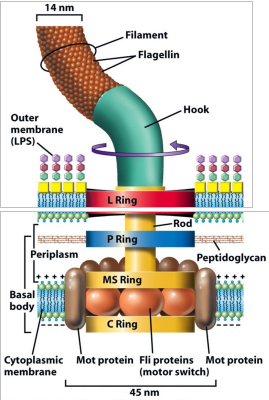
\includegraphics[scale=0.7]{img/Flagello.png}
\caption{Struttura dei flagelli batterici}
\label{}
\end{figure}


\subsubsection{Il flagello dei Gram+}

Nei Gram+ i dischi sono solo due:
\begin{enumerate}
\item un \textbf{anello P}, associato al peptidoglicano;
\item un \textbf{anello M}, associato alla membrana plasmatica.
\end{enumerate}

\subsection{La sintesi del flagello}

La sintesi del flagello nei batteri è regolata da \emph{3 operoni} e \emph{60 geni}.
Essa si svolge in 3 fasi:
\begin{enumerate}
\item l’\textbf{operone di classe I (flhDC)} viene trascritto e si forma un complesso eteromultimerico che ha la funzione di sintetizzare una proteina con funzione di attivatore trascrizionale che attiva la trascrizione dell’operone di classe II;
\item l’\textbf{operone di classe II} attivato codifica per proteine strutturali del corpo basale e dell’uncino, e va ad attivare l’operone di classe III;
\item l’\textbf{opero di classe III} va a sintetizzare proteine del filamento (monomeri di flagellina), del motore flagellare MOT, e proteine per il sistema di trasduzione del segnale della chemiotassi.
\end{enumerate}

I monomeri di flagellina vengono sintetizzati nel citoplasma, passano all’interno del canale del flagello e si attaccano all’apice dei monomeri del flagello in sintesi (autoassemblaggio).

\begin{figure}[htp]
\centering
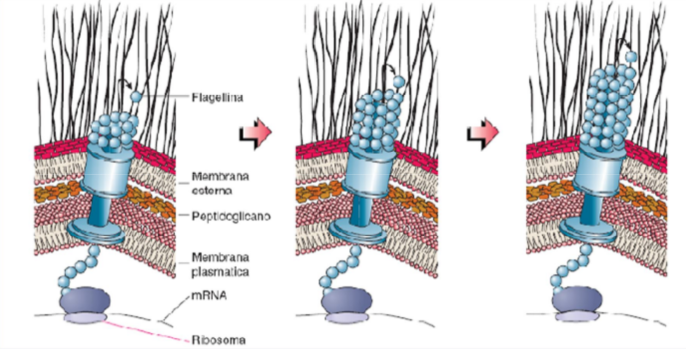
\includegraphics[scale=0.5]{img/Assemblaggio flagello.png}
\caption{Assemblaggio del flagello}
\label{}
\end{figure}


\subsection{Il movimento dei flagelli}

Il movimento di una cellula flagellata è impartito dalla rotazione del filamento:le cellule monotriche possono muoversi in avanti ruotando il flagello in senso antiorario, oppure indietro ruotando il flagello in senso orario. Nelle cellule peritriche o lofotriche (cellule dotate di più flagelli) invece, i flagelli devono essere un po’ riuniti e tutti coordinati nel fare la stessa cosa: se il batterio deve muoversi in avanti i flagelli si uniscono in fasci e danno forza propulsiva al batterio, mentre se il batterio deve cambiare la propria direzione i flagelli si aprono e ruotano in senso orario facendo sì che il batterio compia delle capriole che ne cambiano l’orientamento nello spazio.

\vspace{1em}
La produzione di energia, così come il movimento batterico, avviene grazie ad un flusso di protoni attraverso la membrana plasmatica che crea un gradiente di concentrazione \emph{(forza proton motrice)}: questo gradiente induce una \emph{modificazione strutturale nella proteina MotA} che circonda i dischi situati più all’interno della membrana.\\
Le proteine Mot imprimono un movimento rotatorio alle proteine FliG, le quali sono compattate fra i dischi MS e C. Questo movimento fa sì che lo spostamento dei dischi venga trasmesso all’albero motore, all’uncino, ed infine al flagello.\\
Il rotore può fare dai 6.000 ai 17.000 giri al minuto, ma il filamento arriva solo a 200 – 1.000 giri al minuto (rpm). Ogni giro richiede all’incirca lo spostamento di 1.000 protoni.

I flagelli degli Archea
Il flagello degli Archaea è simile a quello degli Eubatteri. 
Le principali differenze sono:
1. I flagelli batterici si muovono grazie ad una forza proton motrice, quelli degli Archaea si muovono grazie all’ATP;
2. Le cellule batteriche hanno molti filamenti flagellari ognuno dei quali ruota indipendentemente, il flagello degli Archaea si compone di pacchetti di filamenti che ruotano come se fossero assemblati insieme;
3. I flagelli batterici crescono mediante aggiunta di monomeri di flagellina all’apice del flagello, quelli degli Archaea crescono per aggiunta di flagellina nella zona basale e il flagello viene spinto fuori;
4. I flagelli batterici sono più spessi di quelli degli Archaea.

Batteri particolari: le spirochete (Gram -).
Le spirochete sono batteri bastoncellari a forma elicoidale. 
Questi batteri possiedono un flagello interno, periplasmatico, invece che uno esterno.
Questa posizione del flagello rende il movimento delle spirochete particolare: esse “ruotano” su se stesse, attorcigliandosi come delle viti.
La rotazione dei filamenti flagellari induce la rotazione e la deformazione dinamica della cellula
che spinge il batterio attraverso il fluido.
Nelle spirochete rigide (Treponema) la rotazione dei flagelli induce un movimento a spirale, mentre nelle
spirochete flessibili (Borrelia) induce una curvatura e movimento a spirale.
o alla membrana plasmatica.

Il movimento di una cellula flagellata è impartito dalla rotazione del filamento:
Le cellule monotriche possono muoversi in avanti ruotando il flagello in senso antiorario, indietro ruotando il flagello in senso orario;
Nelle cellule peritriche o lofotriche, cioè quelle cellule dotate di più flagelli, questi devono essere un po’ riuniti e tutti coordinati nel fare la stessa cosa. Se il batterio deve muoversi in avanti i flagelli si uniscono in fasci e danno forza propulsiva al batterio, mentre se il batterio deve cambiare la propria direzione i flagelli si apriranno e ruoteranno in senso orario facendo sì che il batterio compia delle capriole che ne cambino l’orientamento nello spazio.

La sintesi del flagello nei batteri è regolata da 3 operoni e 60 geni.
Essa si svolge in 3 fasi:
1. L’operone I (flhDC) viene trascritto e si forma un complesso eteromultimerico che ha la funzione di sintetizzare una proteina con funzione di attivatore trascrizionale che attiva la trascrizione dell’operone di classe II;
2. L’operone di classe II attivato codifica per proteine strutturali del corpo basale e dell’uncino, e va ad attivare l’operone di classe III;
3. L’opero di classe III va a sintetizzare proteine del filamento (monomeri di flagellina), del motore flagellare MOT, e proteine per il sistema di trasduzione del segnale della chemiotassi.

I monomeri di flagellina vengono sintetizzati nel citoplasma, passano all’interno del canale del flagello e si attaccano all’apice dei monomeri del flagello in sintesi (autoassemblaggio).

Come si muovono i flagelli?
La produzione di energia così come il movimento batterico, avviene grazie ad un flusso di protoni attraverso la membrana plasmatica che crea un gradiente di concentrazione (forza proton motrice): questo gradiente induce una modificazione strutturale nella proteina MotA che circonda i dischi situati più all’interno della membrana. Le proteine Mot imprimono un movimento rotatorio alle proteine FliG, le quali sono compattate fra i dischi MS e C. Questo movimento fa sì che lo spostamento dei dischi venga trasmesso all’albero motore, all’uncino, ed infine al flagello.
Il rotore può fare dai 6.000 ai 17.000 giri al minuto, ma il filamento arriva solo a 200 – 1.000 giri al minuto (rpm): ogni giro richiede all’incirca lo spostamento di 1.000 protoni.






















\end{document}